\section{Introduction}

The purpose of this paper is to report on the \emph{Equational Theories Project} (ETP)\footnote{\url{https://teorth.github.io/equational_theories/}}, a pilot project launched\footnote{\url{https://terrytao.wordpress.com/2024/09/25}} in September 2024 to explore new ways to collaboratively work on mathematical research projects using machine assistance. The project goal, in the area of universal algebra, was selected\footnote{The specific mathematical goal was inspired by \href{https://mathoverflow.net/questions/450930}{a MathOverflow question}.} to be particularly amenable to crowdsourced and computer-assisted techniques, while still being of mathematical research interest.

The project achieved its primary goal on 14 April 2025, when the $\num{4694} \times (\num{4694}-1) = \num{22028942}$ implications between the test set of $\num{4964}$ equational laws were completely determined, with proofs or refutations formalized in \emph{Lean}.  This required coordinating the efforts of a large number of participants contributing both human-written formalizations and automatically generated proofs from various computer tools.  In this paper, we report on both the scientific outcomes of the project, as well as the organizational issues that came up with organizing a mathematical project of this scale.

\subsection{Magmas and Equational Laws}

In order to describe the mathematical goals of the ETP, we need some notation. A \emph{magma} $\Magma = (M,\op)$ is a set $M$ (known as the \emph{carrier}) together with a binary operation $\op \colon M \times M \to M$. An \emph{equational law} for a magma, or \emph{law} for short, is an identity involving $\op$ and some formal indeterminates, which we will typically denote using the Roman letters $\x,\y,\z,\w,\uu,\vv$, as well as the formal equality symbol $\formaleq$ in place of the equality symbol $=$ to emphasize the formal nature of the law.

In the ETP, a unique number was assigned to each equational law, via a numbering system that we describe in \Cref{numbering-app}.  For instance, the \emph{commutative law} $\x \op \y \formaleq \y \op \x$ is assigned the equation number \eqref{eq43}, while the \emph{associative law} $(\x \op \y) \op \z \formaleq \x \op (\y \op \z)$ is assigned the equation number \eqref{eq4512}.  A list of all equations referred to by number in this paper is also provided in \Cref{numbering-app}.

A magma $\Magma = (M,\op)$ obeys a law $E$ if the law $E$ holds for all possible assignments of the indeterminate to elements of $M$, in which case we write $\Magma \models E$. Thus, for instance $\Magma \models \Eq{43}$ if one has $x \op y = y \op x$ for all $x,y \in M$.  Note that the formal indeterminate symbols $\x, \y$ in $\Eq{43}$ are now replaced by concrete elements $x,y$ of the carrier $M$.

We say that a law $E$ \emph{entails} or \emph{implies} another law $E'$ if every magma that obeys $E$, also implies $E'$: $(\Magma \models E) \implies (\Magma \models E')$.  We write this relation as $E \vdash E'$. We say that two laws are \emph{equivalent} if they entail each other. For instance, the constant law $\x \op \y \formaleq \z \op \w$ \eqref{eq46} can easily be seen to be equivalent to the law $\x \op \x \formaleq \y \op \z$ \eqref{eq41}.  It is clear that $\vdash$ is a pre-order, that is to say a partial order after one quotients by equivalence.

In this entailment pre-ordering, the maximal element is given by the trivial law $\x\formaleq\x$ \eqref{eq1}, and the minimal element is given by the singleton law $\x\formaleq \y$ \eqref{eq2}, thus $\Eq{2} \vdash E \vdash \Eq{1}$ for all laws $E$.

We also define a variant: we say that $E$ \emph{entails} $E'$ \emph{for finite magmas}, and write $E \vdashfin E'$, if every \emph{finite} magma $M$ that obeys $E$, also obeys $E'$.  Clearly, the relation $E \vdash E'$ implies $E \vdashfin E'$; but, as observed by Austin \cite{austin_finite}, the converse is not true in general.

The \emph{order} of an equational law is the number of occurrences of the magma operation, and can be viewed as a crude measure of complexity of the law. For instance, the commutative law \eqref{eq43} has order $2$, while the associative law \eqref{eq4512} has order $4$. We note some selected laws of small order that have previously appeared in the literature:
\begin{itemize}
\item The \emph{central groupoid law} $\x \formaleq (\y \op \x) \op (\x \op \z)$ \eqref{eq168} is an order-$3$ law introduced by Evans \cite{evans} and studied further by Knuth \cite{knuth} and many further authors, being closely related to central digraphs (also known as unique path property diagraphs), and leading in particular to the discovery of the Knuth-Bendix algorithm \cite{knuth-bendix}; see \cite{klt} for a more recent survey.
\item \emph{Tarski's axiom} $\x \formaleq \y \op (\z \op (\x \op (\y \op \z)))$ \eqref{eq543} is an order-$4$ law that was shown by Tarski \cite{Tarski1938} to characterize the operation of subtraction in an abelian group; that is to say, a magma $\Magma = (M,\op)$ obeys \eqref{eq543} if and only if there is an abelian group structure on $\Magma$ for which $x \op y = x-y$ for all $x,y \in M$.
\item In a similar vein, it was shown in \cite{mendelsohn-padmanabhan} (see also \cite{meredith-prior}) that the order-$4$ law
$\x \formaleq (\y \op \z) \op (\y \op (\x \op \z))$ \eqref{eq1571} characterizes addition (or subtraction) in an abelian group of exponent $2$; it was shown in \cite{mccune_et_al} that the order-$6$ law $\x \formaleq (\y \op ((\x \op \y) \op \y)) \op (\x \op (\z \op \y))$ \eqref{eq345169} characterizes the Sheffer stroke in a boolean algebra, and it was shown in \cite{higman-neumann} that the order-$8$ law
$\x \formaleq \y \op ((((\y \op \y) \op \x) \op \z) \op (((\y \op \y) \op \y) \op \z))$ \eqref{eq42323216} characterizes division in a (not necessarily abelian) group.
\end{itemize}
Some further examples of laws characterizing well-known algebraic structures are listed in \cite{mccune-survey}.

The Birkhoff completeness theorem \cite[Th.~3.5.14]{term-rewriting} implies that an implication $E \vdash E'$ of equational laws holds if and only if the left-hand side of $E'$ can be transformed into the right-hand side by a finite number of substitution rewrites using the law $E$. However, the problem of determining whether such an implication holds is undecidable in general \cite{mckenzie}. Even when the order is small, some implications\footnote{Another contemporaneous example of this phenomenon was the solution of the Robbins problem \cite{robbins}.} can require lengthy computer-assisted proofs; for instance, it was noted in \cite{Kisielewicz2} that the order-$4$ law $\x \formaleq (\y \op \x) \op ((\x \op \z) \op \z)$ \eqref{eq1689} was equivalent to the singleton law \eqref{eq2}, but all known proofs were found with computer assistance.\footnote{We improved such a proof to make it human-readable, see \href{https://teorth.github.io/equational_theories/blueprint/implications-chapter.html}{the blueprint of the ETP}.}  Furthermore, for the finite magma implication relation $E \vdashfin E'$, no analogue of the Birkhoff completeness theorem is available.

\subsection{The Equational Theories Project}

As noted in \Cref{numbering-app}, there are $\num{4694}$ equational laws of order at most $4$. The primary mathematical goal of the ETP was to completely determine the \emph{implication graph} for these laws, in which there is a directed edge from $E$ to $E'$ precisely when $E \vdash E'$. As the project progressed, an additional goal was added to determine the slightly larger \emph{finite implication graph}, in which there is a directed edge from $E$ to $E'$ precisely when $E \vdashfin E'$.

Such systematic determinations of implication graphs have been seen previously in the literature; for instance, in \cite{phillips-vojtechovsky}, the relations between $60$ identities of Bol--Moufang type were established, and in the blog post \cite[\S 17]{Wolfram_2022}, some initial steps towards generating this graph for the first hundred or so laws on our list were performed. However, to our knowledge, the ETP is the first project to study such implications at the scale of thousands of laws.

The ETP requires the determination of the truth or falsity of $\num{4694}^2 = \num{22033636}$ implications (for both arbitrary magmas and finite magmas), or $\num{4694} \times (\num{4694}-1) = \num{22028942}$ if the reflexive implications $E \vdash E$ are removed; while one can use properties such as the transitivity of entailment to reduce the work somewhat, this is clearly a task that requires significant automation. It was also a project highly amenable to crowdsourcing, in which different participants could work on developing different techniques, each of which could be used to fill out a different part of the implication graph. In this respect, the project could be compared with a Polymath project \cite{Gowers2009}, which used online forums such as blogs and wikis to openly collaborate on a mathematical research problem. However, the Polymath model required human moderators to review and integrate the contributions of the participants, which clearly would not scale to the ETP which required the verification of over twenty million mathematical statements. Instead, the ETP was centered around a GitHub repository in which the formal mathematical contributions had to be entered in the proof assistant language \emph{Lean}, where they could be automatically verified. In this respect, the ETP was more similar to the recently concluded Busy Beaver Challenge\footnote{\url{https://bbchallenge.org/}}, which was a similarly crowdsourced project that computed the fifth Busy Beaver number $BB(5)$ to be $\num{47176870}$ through an analysis of about $180$ million Turing machines, with the halting analysis being verified in a variety of computer languages, with the final formal proof written in the proof assistant language \emph{Coq} \cite{the_coq_development_team_2024_14542673, bbchallenge_bb5}. One of the aims of the ETP was to explore potential workflows for such collaborative, formally verified mathematical research projects that could serve as a model for future projects of this nature.

Secondary aims of the ETP included the possibility of discovering unusually interesting equational laws, or new experimental observations about such laws, that had not previously been noticed in the literature; and to develop benchmarks to assess the performance of automated theorem provers and other AI tools.

\subsection{Outcomes}

The ETP achieved almost all of its primary objectives, with all of the $\num{22033636}$ implications $E \vdash E'$ and non-implications $E \not \vdash E'$ magmas formalized in the proof assistant language \emph{Lean}, and can be found on the ETP GitHub repository.  See \Cref{fig:854}, \Cref{fig:1729} and \Cref{fig:longchain} for some small fragments of the implication graphs produced.
The $\num{4694}$ laws organized into $\num{1415}$ equivalence classes, with by far the largest class being the class of $\num{1486}$ equations equivalent to the trivial law $\Eq{2}$.

For the finite implication graph $E \vdashfin E'$, we could similarly formalize all but two implications.  Specifically, we were unable to obtain either a human-readable or formalized proof or disproof of the implication $E677 \vdashfin E255$ (or its equivalent dual $E2910 \vdashfin E47$), despite extensive efforts from the participants of the project; we tentatively conjecture this implication to be false (i.e., that there exists a finite magma obeying \eqref{eq677} but not \eqref{eq255}), but the refutation appears to be ``immune'' to most of the techniques that we developed for the project.  (We were however able to establish that the corresponding implication $E677 \vdash E255$ for arbitrary magmas was false, using the greedy construction discussed in \Cref{greedy-sec}.)

\begin{figure}
\centering
\includegraphics[width=0.85\textwidth]{854.png}
\caption{A Hasse diagram of all the equational laws implied by \eqref{eq854} (for unrestricted magmas).  An edge in this diagram indicates that the lower equation implies the higher one. Rounded rectangles indicate groups of equivalent laws.  This graph was produced by the visualization tool \emph{Graphiti}, which was developed for this project.}
\label{fig:854}
\end{figure}

\begin{figure}
    \centering
    \includegraphics[width=0.4\textwidth]{ramanujan-infinite.png}
    \includegraphics[width=0.4\textwidth]{ramanujan-finite.png}
    \caption{A Hasse diagram of all the equational laws implied by \eqref{eq1729}, both for unrestricted magmas (left) and finite magmas (right). Note the slightly larger number of implications in the latter.}
    \label{fig:1729}
\end{figure}

\begin{figure}
    \centering
    \resizebox{\textwidth}{!}{%
      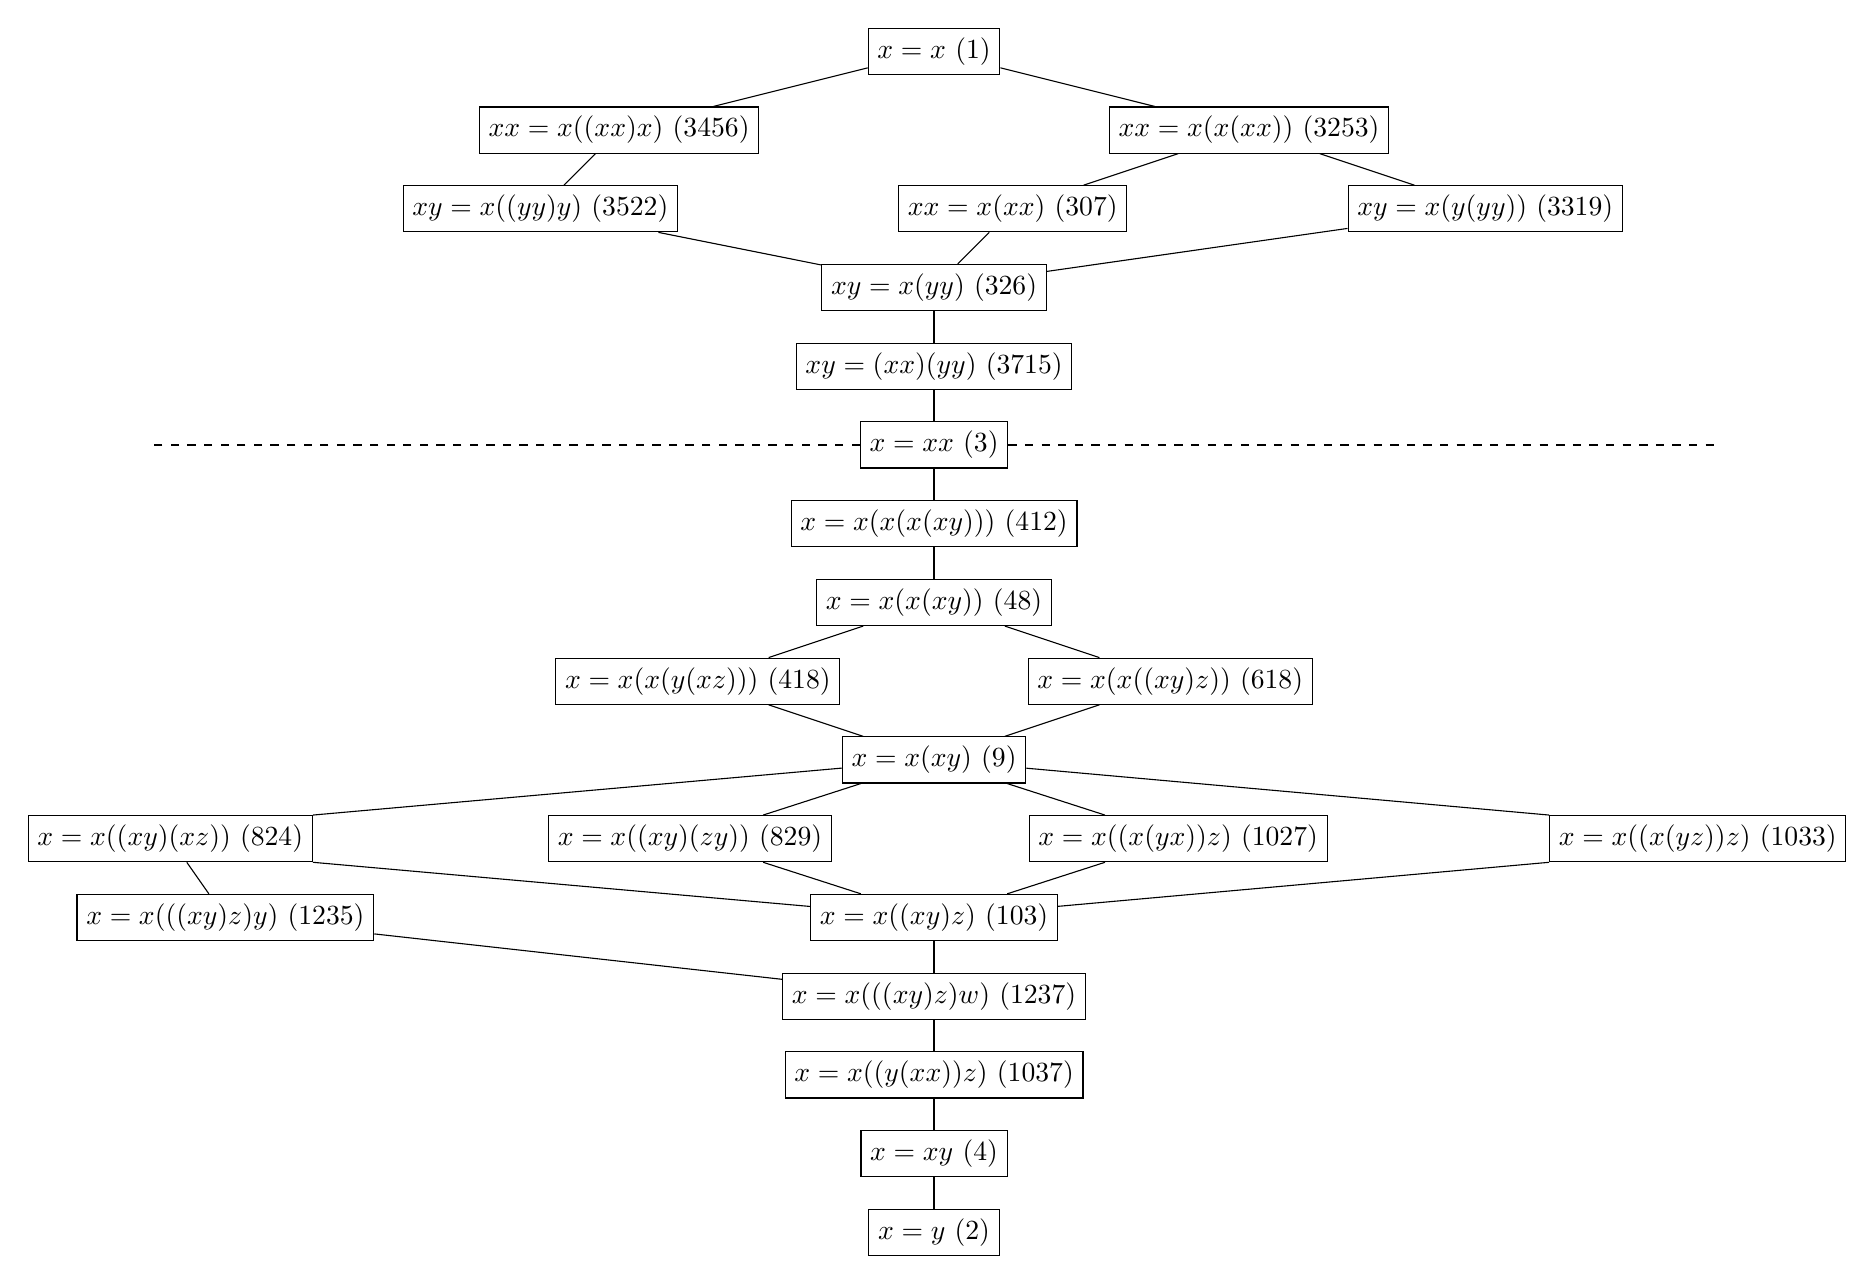
\begin{tikzpicture}
        \node(1)[draw] at (0,15) {$x = x$ (1)};
        \node(3253)[draw] at (4,14) {$x \op x = x \op (x \op (x \op x))$ (3253)};
        \node(3456)[draw] at (-4,14) {$x \op x = x \op ((x \op x) \op x)$ (3456)};
        \node(3319)[draw] at (7,13) {$x \op y = x \op (y \op (y \op y))$ (3319)};
        \node(307)[draw] at (1,13) {$x \op x = x \op (x \op x)$ (307)};
        \node(3522)[draw] at (-5,13) {$x \op y = x \op ((y \op y) \op y)$ (3522)};
        \node(326)[draw] at (0,12) {$x \op y = x \op (y \op y)$ (326)};
        \node(3715)[draw] at (0,11) {$x \op y = (x \op x) \op (y \op y)$ (3715)};
        \node(3)[draw] at (0,10) {$x = x \op x$ (3)};
        \draw[dashed](3)--(-10,10);
        \draw[dashed](3)--(10,10);
        \node(412)[draw] at (0,9) {$x = x \op (x \op (x \op (x \op y)))$ (412)};
        \node(48)[draw] at (0,8) {$x = x \op (x \op (x \op y))$ (48)};
        \node(618)[draw] at (3,7) {$x = x \op (x \op ((x \op y) \op z))$ (618)};
        \node(418)[draw] at (-3,7) {$x = x \op (x \op (y \op (x \op z)))$ (418)};
        \node(9)[draw] at (0,6) {$x = x \op (x \op y)$ (9)};
        \node(824)[draw] at (-9.7,5) {$x = x \op ((x \op y) \op (x \op z))$ (824)};
        \node(829)[draw] at (-3.1,5) {$x = x \op ((x \op y) \op (z \op y))$ (829)};
        \node(1027)[draw] at (3.1,5) {$x = x \op ((x \op (y \op x)) \op z)$ (1027)};
        \node(1033)[draw] at (9.7,5) {$x = x \op ((x \op (y \op z)) \op z)$ (1033)};
        \node(103)[draw] at (0,4) {$x = x \op ((x \op y) \op z)$ (103)};
        \node(1235)[draw] at (-9,4) {$x = x \op (((x \op y) \op z) \op y)$ (1235)};
        \node(1237)[draw] at (0,3) {$x = x \op (((x \op y) \op z) \op w)$ (1237)};
        \node(1037)[draw] at (0,2) {$x = x \op ((y \op (x \op x)) \op z)$ (1037)};
        \node(4)[draw] at (0,1) {$x = x \op y$ (4)};
        \node(2)[draw] at (0,0) {$x = y$ (2)};
        \draw(2)--(4);
        \draw(4)--(1037);
        \draw(1037)--(1237);
        \draw(1237)--(1235);
        \draw(1235)--(824);
        \draw(1237)--(103);
        \draw(103)--(1027);
        \draw(103)--(1033.south west);
        \draw(103)--(824.south east);
        \draw(103)--(829);
        \draw(1027)--(9);
        \draw(1033.north west)--(9);
        \draw(829)--(9);
        \draw(824.north east)--(9);
        \draw(9)--(418);
        \draw(9)--(618);
        \draw(418)--(48);
        \draw(618)--(48);
        \draw(48)--(412);
        \draw(412)--(3);
        \draw(3)--(3715);
        \draw(3715)--(326);
        \draw(326)--(3522);
        \draw(3522)--(3456);
        \draw(3456)--(1);
        \draw(326)--(307);
        \draw(307)--(3253);
        \draw(3253)--(1);
        \draw(326)--(3319);
        \draw(3319)--(3253);
      \end{tikzpicture}%
    }
    \caption{Longest chains of implications (length $15$) between inequivalent laws in the implication graph.  The parts above/below law 3 can be independently dualized. }
    \label{fig:longchain}
\end{figure}

Of the $\num{22033636}$ possible implications $E \vdash E'$, $8178279$ (or $37.12\%$) would end up being true; for an additional set of either $820$ or $822$ pairs $E,E'$, the weaker implication $E \vdashfin E'$ also held. To establish such positive implications $E \vdash E'$ or $E \vdashfin E'$, the main techniques used were as follows:

\begin{itemize}
    \item A very small number of positive implications were established and \textbf{formalized by hand}, mostly through direct rewriting of the laws; but this approach would not scale to the full project.
    \item \textbf{Simple rewriting rules}, for instance based on the observation that any law of the form $\x \formaleq f(\y,\z,\dots)$ was necessarily equivalent to the trivial law \eqref{eq2}, could already reduce the size of potential equivalence classes by a significant fraction. We discuss this method in \Cref{rewrite-sec}.
    \item The preorder axioms for $\vdash$, as well as the ``duality'' symmetry of the preorder with respect to replacing a magma operation $x \op y$ with its opposite $x \op^{\mathrm{op}} y \coloneqq y \op x$, can be used to significantly cut down on the number of implications that need to be proven explicitly; ultimately, only $10657$ ($0.05\%$) of the positive implications needed a direct proof.
    \item To obtain additional implications for finite magmas, heavy reliance was made on the fact that for functions $f \colon M \to M$ on a finite set $M$, surjectivity was equivalent to injectivity.  Some more sophisticated variants of this idea can lead to additional implications; see \Cref{finite-sec}.
    \item \textbf{Automated Theorem Provers} (ATP) could be deployed at extremely fast speeds to establish a complete generating set of positive implications; see \Cref{automated-sec}.
\end{itemize}

More challenging were the $\num{13855357}$ ($62.88\%$) implications that were false, $E \nvdash E'$, and particularly the slightly smaller set of $\num{13854535}$ or $\num{13854537}$ implications that were false even for finite magmas, $E \nvdashfin E'$. Here, the range of techniques needed to refute such implications were quite varied, and may be of independent interest:
\begin{itemize}
        \item \textbf{Syntactic methods}, such as observing a ``matching invariant'' of the law $E$ that was not shared by the law $E'$, could be used to obtain some refutations.  For instance, if both sides of $E$ had the same order, but both sides of $E'$ did not, this could be used to syntactically refute $E \vdash E'$.  Similarly, if the law $E$ was confluent, enjoyed a complete rewriting system, or otherwise permitted some understanding of the free magma associated to that law, one could decide the assertions $E \vdash E'$ for all possible laws $E'$, or at least a significant fraction of such laws.  We discuss these methods, and the extent to which they can be automated, in \Cref{syntactic-sec}.
        \item \textbf{Small finite magmas}, which can be described explicitly by multiplication tables, could be tested by brute force computations to provide a large number of finite counterexamples to implications, or by ATP-assisted methods. See \Cref{finite-sec}.
        \item \textbf{Linear models}, in which the magma operation took the form $x \op y = ax + by$ for some (commuting or non-commuting) coefficients $a,b$, allowed for another large class of counterexamples to implications, which could be automatically scanned for either by brute force or by Grobner basis type calculations; many of these examples could also be made finite. See \Cref{linear-sec}.
        \item \textbf{Translation invariant models}, in which the magma operation took the form $x \op y = x + f(y-x)$ on an additive group, or $x \op y = x f(x^{-1} y)$ on a non-commutative group, reduce matters to analyzing certain functional equations; see \Cref{translation-sec}.
        \item \textbf{Greedy methods}, in which either the multiplication table $(x,y) \mapsto x \op y$ or the function $f$ determining a translation-invariant model are iteratively constructed by a greedy algorithm subject to a well-chosen ruleset, were effective in resolving many implications not easily disposed of by preceding methods. See \Cref{greedy-sec}.
        \item Starting with a simple base magma $\Magma$ obeying both $E$ and $E'$, and either \textbf{enlarging} it to a larger magma $\Magma'$ containing $\Magma$ as a submagma, \textbf{extending} it to a magma $\MagmaN$ with a projection homomorphism $\pi: \MagmaN \to \Magma$, or \emph{modifying the multiplication table} on a small number of values, also proved effective when combined with greedy methods or with a ``\textbf{magma cohomology}'' construction. See \Cref{modify-base}.
        \item To each equation $E$ one can associate a ``\textbf{twisting semigroup}'' $S_E$.  If $S_E$ is larger than $S_{E'}$, then this can often be used to disprove the implication $E \vdash E'$; see \Cref{twisting-sec}.
        \item Some \textbf{ad hoc models} based on existing mathematical objects, such as infinite trees, rings of polynomials, or ``Kisielewicz models'' utilizing the prime factorization of the natural numbers, could also handle some otherwise difficult cases.  In some cases, the magma law induced some relevant and familiar structures, such as a directed graph or a partial order, which also helped guide counterexample constructions. We will not detail these diverse examples here, but refer the reader to the ETP blueprint for more discussion.
        \item \textbf{Automated theorem provers} were helpful in identifying which simplifying axioms could be added to the magma without jeopardizing the ability to refute the desired implication $E \vdash E'$ or $E \vdashfin E'$.
\end{itemize}

While the vast majority of negative implications could be quickly resolved by one of the above techniques, either with human input or in a completely automated fashion, there were perhaps two dozen such negative results that required quite delicate and \emph{sui generis} constructions.  The hardest such implication, $\Eq{1729} \nvdash \Eq{817}$, took several months to establish and then formalize (using a combination of many of the above constructions), with the final proof in \emph{Lean} requiring just over $\num{4000}$ dedicated lines of code from multiple contributors.

In the course of completing the implication graph, some interesting new algebraic structures were discovered.  One such example concerns the magmas obeying \eqref{eq1485}, which we refer to as \emph{weak central groupoids} as they contain the central groupoids (obeying \eqref{eq168}) as a subclass.  In \cite{knuth} it was observed that all finite central groupoids have order equal to a perfect square $n^2$; empirically, we have found that finite weak central groupoids always have order $n^2$ or $2n^2$, although we have no rigorous proof of this claim; they also have a graph-theoretic interpretation analogous to the interpretation of central groupoids as digraphs with the unique path property.  For these and other observations we refer the reader to \href{https://teorth.github.io/equational_theories/blueprint/weak-central-groupoids-chapter.html}{the blueprint of the ETP}.

The objective of using the data from the ETP to establish well-calibrated benchmarks to evaluate ATPs remains an interesting open problem; the participants of this project did not have the required expertise to develop and test such benchmarks to the standards expected in the area.  However, in \Cref{automated-sec} we present a more informal ``field report'' of our experiences using ATPs in the project, in the hope that this will provide some useful guidance to other researchers seeking to incorporate ATPs into their own research.

\begin{figure}
\centering
\begin{tikzpicture}[
    >=Latex,
    node distance=1.3cm,
    every node/.style={draw, rectangle, align=center},
    label/.style={font=\bfseries}
  ]

  %% Column labels
  \node[label] (ghlabel)   at (0,2) {GitHub};
  \node[label] (zuliplabel) at (7,2) {Lean Zulip};

  %% GitHub nodes
  \node (blueprint)   {Blueprint};
  \node (formal)     [below=of blueprint] {Lean formalization};
  \node (viz)        [below=of formal]    {Visualization tools};

  %% Lean Zulip nodes
  \node (hproofs)    [right=of blueprint]       {Human-generated proofs};
  \node (cproofs)    [right=3cm of formal]         {Computer-generated proofs};
  \node (hdisc)      [right=of viz]         {Human discussion};

  %% External ATP box
  \node (atp)        [right=of cproofs]         {ATPs and other\\external software tools};

  %% Grouping boxes
  % GitHub container
  \node[draw,dotted,inner sep=8pt,fit=(blueprint)(formal)(viz), label=above:GitHub]
    (ghbox) {};
  % Lean Zulip container
  \node[draw,dotted,inner sep=8pt,fit=(hproofs)(cproofs)(hdisc), label=above:Lean Zulip]
    (zulipbox) {};

  %% Arrows
  \draw[human,->] (blueprint)  -- (formal);
  \draw[auto,->] (formal)     -- (viz);
  \draw[human,->] (viz)        -- (hdisc);
  \draw[human,->] (hdisc)      -- (atp);
  \draw[auto,->] (atp)        -- (cproofs);
  \draw[human,->] (cproofs)    -- (hproofs);
  \draw[semi,->] (cproofs)    -- (formal);
  \draw[human,<->] (hproofs)   -- (hdisc);
  \draw[human,->] (hproofs)  -- (blueprint);
  \draw[human,->] (hproofs)  -- (formal);

\end{tikzpicture}
\caption{Some of the main dynamics in which proofs were generated, discussed within the Lean Zulip channel and then formalized in the Github repository.  Boldface arrows indicate human activities, such as proposing an automated attack on outstanding implications, converting a computer-generated proof into a human-readable format, formalizing a human readable proof directly, or first creating a more precise blueprint for other collaborators to work on.  Dashed arrows indicate fully automated processes, while the partly dashed line indicated a semi-automated process requiring human supervision. }
\label{fig:flow}
\end{figure}

\subsection{Further directions}

While the primary objective of the ETP was being completed, some additional related results were generated as spinoffs.  Specifically:
\begin{itemize}
\item In the blueprint on the ETP web site, we report some partial progress on classifying which of the $57882$ distinct laws of order $5$ are equivalent to the singleton law \eqref{eq2}, either with or without the requirement that the magma be finite.
\item In \Cref{higman-neumann} we report on classifying the laws of order $8$ that are equivalent to the Higman-Neumann law \eqref{eq42323216}.
\item In \Cref{ml-sec} we report on preliminary experiments on using machine learning to determine to what extent the implication graph can be predicted by a neural network.
\end{itemize}
